\chapter{A Dynamic Navigation Model for Co-located Collaboration}
\label{chapter:dynamic_model}
\pagebreak

\textbf{Chapter Abstract}

This chapter presents a novel dynamic navigation model that we design for co-located collaboration. This model manages user cohabitation by integrating constrains from physical workspace and allows interactive navigation control by adding virtual constrains. First we explain our motivation and different components of the dynamic model at the conceptual level, then we present implementation details from data structure to code organization, as well as some discussions about possible future improvements.

\vspace*{2\baselineskip}

\minitoc

\newpage
\section{Introduction}
The Altered Human Joystick metaphor allows individual navigation for multiple users, however, each user is constrained in a predefined safe zone and the common workspace is shared by using a system dependent protocol (which works for CAVE-like immersive systems). Moreover, in many rate control navigation metaphors, the virtual vehicle's velocity is exclusively controlled by user's input and can not be influenced by constrains from the virtual world (e.g. collisions with objects). 

To generalize the Altered Human Joystick metaphor and to allow interactive control of the virtual vehicle, we designed a dynamic navigation model named DYNAMIC (DYnamic NAvigation Model for Immersive Collaboration), which on the one hand, integrates real world information into the virtual navigation control to manage user cohabitation no matter the geometric properties of the immersive system, and on the other hand, takes into account influences coming from the virtual world and eventually from the vehicles of other users.

This chapter mainly contains four sections. The first section explains our motivation of developing this dynamic navigation model. The second part describes core concepts of this model: the acceleration-based transfer function and how we integrate constrains coming from the physical workspace and the virtual world. Then the third section presents implementation details and the last one some related discussion about this navigation model.

% -------------------------------------------------------------------------------------------------

\section{Motivation}
The dynamic navigation model is the result of responses to two different research questions that we are working on: how can we generalize the Altered Human Joystick metaphor to extend the number of users regardless of the geometric configuration of immersive systems? And how can we make the virtual vehicle to be responsive to constrains coming from the virtual world to achieve interactions with virtual objects and other users during navigation?

This new model is dynamic because the transfer functions used in human joystick metaphors are replaced by their derivatives, so the vehicle is controlled by accelerations instead of setting directly its navigation velocity. As a consequence, the virtual vehicle is transformed from a pure reference frame to a virtual entity possessing its own kinematic state, providing a uniform interface to receive inputs from various sources. First, to integrate constrains from the physical workspace, we use a potential field method that generates accelerations for the virtual vehicle in order to influence user's navigation control. Second, virtual vehicles can now react to constrains in the virtual worlds in form of physical links. We can simulate physical interactions between a vehicle and virtual objects, or directly between different users' vehicles during navigation. 


% -------------------------------------------------------------------------------------------------


\section{Concepts}

\subsection{Transfer Function}
The original human joystick metaphor and the altered versions that we present in the previous chapter are based on transfer functions that map a user's relative position and orientation related to a neutral reference frame in the real world to the vehicle's translation and rotation velocities. In this previous model, a neutral position and orientation $(p_{0},q_{0})$ need to be defined before starting navigation. The vehicle's translation and rotation velocity are expressed as:

\begin{equation}
\begin{cases}
\overrightarrow{v_{veh}}=f(\Delta p)=f(p_{u}-p_{0}) \\
\Omega_{veh}=f(\Delta q)=f(q_{0}^{-1} \cdot q_{u})
\end{cases}
\end{equation}

where $p_{u}(x,y,z)$ is user's current position and $q_{u}(q_{x},q_{y},q_{z},q_{w})$ is a quaternion representing user's orientation in the real world.

In the dynamic model, the virtual vehicle is not merely a spatial reference frame, but a virtual entity possessing its own kinematic state. The user input passes from $(\Delta p, \Delta q)$ to their derivatives: 

\begin{equation}
\begin{cases}
\overrightarrow{a_{veh}}=f(\overrightarrow{v_{u}}, \overrightarrow{a_{u}}) \\
\dot{\Omega}_{veh}=f(\omega_{u}, \dot{\omega}_{u})
\end{cases}
\end{equation}

If we define a configuration \textit{c} as the following:

\begin{equation}
c=
\begin{bmatrix}
p \\ q
\end{bmatrix},\:
\dot{c}=
\begin{bmatrix}
\overrightarrow{v} \\ \omega
\end{bmatrix},\:
\ddot{c}=
\begin{bmatrix}
\overrightarrow{a} \\ \dot{\omega}
\end{bmatrix}
\end{equation}

to have a uniform representation of linear and angular information, where $\dot{c}$ and $\ddot{c}$ are the first and second temporal derivatives of \textit{c}. A linear version of the new transfer function can be then expressed as:

\begin{equation}
\ddot{c}_{veh}=K_{1} \cdot \dot{c}_{u} + K_{2} \cdot \ddot{c}_{u}
\end{equation}

\begin{equation}
\begin{bmatrix}
\overrightarrow{a_{veh}} \\ \dot{\omega}_{veh}
\end{bmatrix}=
\begin{bmatrix}
K_{T1} & 0 \\ 0 & K_{R1}
\end{bmatrix}
\begin{bmatrix}
\overrightarrow{v_{u}} \\ \omega_{u}
\end{bmatrix} + 
\begin{bmatrix}
K_{T2} & 0 \\ 0 & K_{R2}
\end{bmatrix}
\begin{bmatrix}
a_{u} \\ \dot{\omega}_{u}
\end{bmatrix}
\end{equation}

Instead of setting directly the vehicle's position or velocity in the virtual world, user's physical movements ``inject" accelerations to animate the virtual vehicle. This transfer function allows easy integration of physical constrains into the vehicle control. Moreover, the navigation velocity no longer depends on user's real world configuration, neither do we need a predefined neutral reference frame.


\subsection{Physical Workspace Constrains}
In a multi-user immersive system, for a given user, the surrounding environment as well as other users are obstacles that should be avoided. Obstacle avoidance is a classical problem in mobile robot motion planning \citep{Latombe2012Robot}. Among all existing methods to guide a robot to navigate over a field occupied by obstacles, potential field method is a commonly used reactive approach that can be easily parameterized and is suitable for real-time processes \citep{Khatib1986Real, Hellstrom2011Robot}.

Generally, two kinds of potential fields lead to two different behaviors of the robot. An attractive field generates an action vector that leads the robot toward the goal, while a repulsive field pushes the robot away from an obstacle. Here we want to use the same principle to guide users by applying repulsive fields to all obstacles in the real world (e.g. screens, walls, other users, etc.). The goal is to keep users away from all the obstacles when they move around in the physical workspace. However, a major problem is that unlike motor-driven robots, users are autonomous actors that can not be directly influenced by the potential field. So, like the divergent transfer function described in the previous chapter (section~\ref{sec:altered_tf}), we modify the output of the transfer function (i.e. $\overrightarrow{a_{veh}}$) by integrating obstacles as real world constrains into the navigation control in order to influence user's input (i.e. $\overrightarrow{v_{u}}$ and $\overrightarrow{a_{u}}$).


\subsubsection{Potential Field}
To achieve the above objective, obstacles generate one potential field for a user's translational movements and another for rotations. The workspace borders are usually fixed while the users are mobile entities, so the global potential fields change dynamically according to users' positions in the physical workspace.

\paragraph{Translation}
To avoid collisions between users and to prevent them from going beyond workspace borders, each physical obstacle produces a repulsive field in which force vectors are in the direction of the surface normal, thus the distribution of potential field depends on obstacles' geometric form. For example, the potential field of a flat wall or screen generates parallel force vectors while those of a user's field (the user is simplified as a cylinder) spread outward from user's position (Figure~\ref{fig:5_pf_t}).

\begin{figure}[htb]
  \centering
  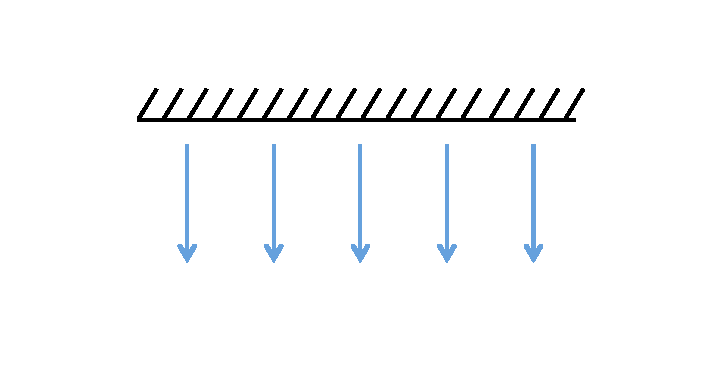
\includegraphics[width=.49\textwidth]{figures/ch5/pf_t_wall}
  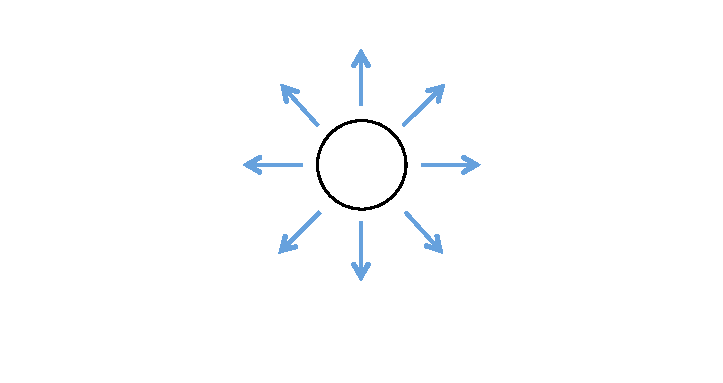
\includegraphics[width=.49\textwidth]{figures/ch5/pf_t_user}
  \caption{\label{fig:5_pf_t}The repulsive translational potential fields generated by obstacles.}
\end{figure}

If we name $\overrightarrow{n_{i}}$ as a unit surface normal vector, $d_{i}$ the distance between a user and the obstacle $i$, the force vector generated for the user $\overrightarrow{ft_{i}}$ can be expressed by a negative exponent function:

\begin{equation}
\overrightarrow{ft}_{i}=\overrightarrow{n}_{i} \cdot K_{T} \cdot \frac{1}{d_{i}^2}
\end{equation}

where $K_{T}$ is a coefficient to modulate the field power.

\paragraph{Rotation}
In projection-based systems, the potential field can help users avoid seeing empty screens and occlusions. Even with HMDs, angular potential fields are still useful if we want to influence a user's orientation in the physical workspace. Angular potential field works in a similar way as for translation, obstacles provide forces to make a user to turn towards one direction or another (clockwise or anti-clockwise). The potential fields associated with screen edges help user stay within projected area, while the potential field of a user pushes other users to look away (Figure~\ref{fig:5_pf_r}).

\begin{figure}[htb]
  \centering
  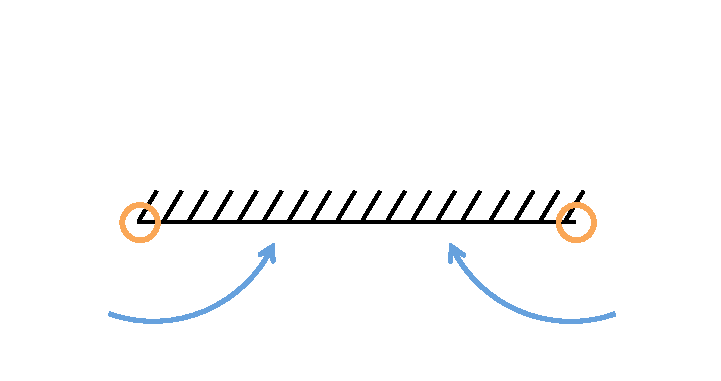
\includegraphics[width=.49\textwidth]{figures/ch5/pf_r_wall}
  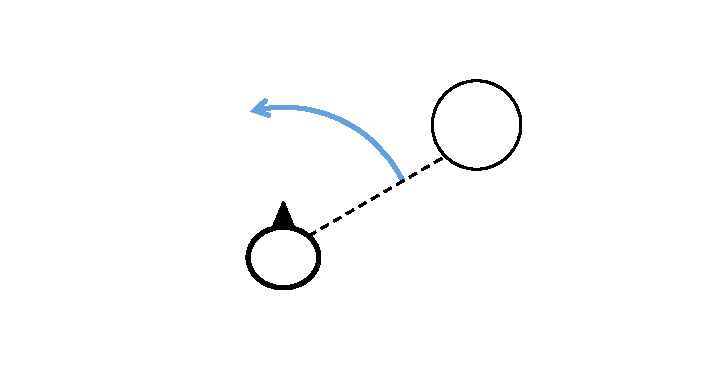
\includegraphics[width=.49\textwidth]{figures/ch5/pf_r_user}
  \caption{\label{fig:5_pf_r}The repulsive angular potential field generated by obstacles.}
\end{figure}

We can name $sign \in \{-1, 1\}$ to indicate the rotation direction (computed using user's orientation compared to the direction vector $\overrightarrow{P_{u}P_{o}}$, $P_{u}$ and $P_{o}$ are respectively the user's and obstacle's position). $\theta_{i}$ is the angle that the user needs to cover starting from the current orientation till seeing the obstacle $i$, then the force vector generated for the user $\overrightarrow{fr}_{i}$ can be expressed by a negative exponent function:

\begin{equation}
{fr}_{i}=sign \cdot K_{R} \cdot \frac{1}{\theta_{i}^2}
\end{equation}

where $K_{R}$ is a coefficient to modulate the field power.

\subsubsection{Solutions}
\label{sec:5_solution}

With the above potential fields associated with each obstacle, users will naturally keep a distance with all obstacles no matter the system configuration, which means we no longer need to specify particular working zones or shared zone for each user as we did in Chapter~\ref{chapter:user_cohab}. So now the question is how users can ``perceive" and be influenced by the potential fields.

\paragraph{Optimal Configuration} In a physical workspace filled with several obstacles, the global potential field for a user is the combination of potential fields of all obstacles, and each user will have a different potential field distribution since he/she is considered as an obstacle for the other users. For each user, the superimposed potential fields result in one or several (local minimum values) special positions and orientations where the forces are neutralized. We can use optimal configuration $c_{opt}$ to denote the combination of optimal position and orientation:

\begin{equation}
c_{opt}=
\begin{bmatrix}
p_{opt} \\ q_{opt}
\end{bmatrix}
\end{equation}

where

\begin{equation}
\sum \overrightarrow{ft}_{i}=[0, 0]\; and\; \sum fr_{i}=0
\end{equation}


Figure~\ref{fig:5_pf_total} shows an example inside a three-wall CAVE, the final potential field for user A is the combination of the fields of other two users and those of all physical borders (a virtual back wall is added to assure users in the range of the screen floor). Optimal position and orientation are marked by green color.

\begin{figure}[htb]
  \centering
  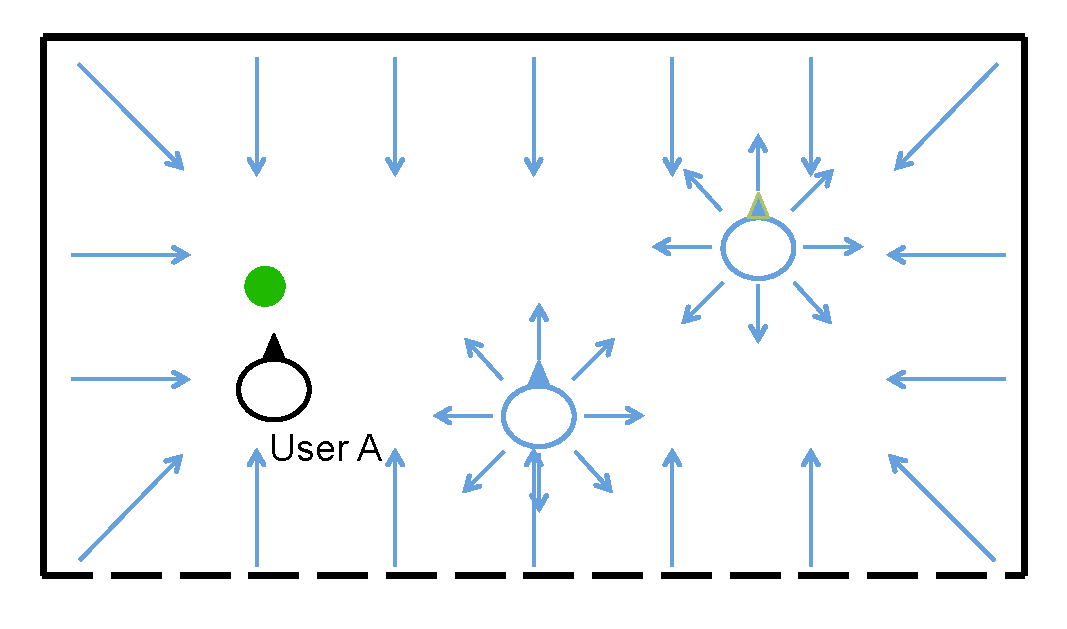
\includegraphics[width=.49\textwidth]{figures/ch5/pf_t_total}
  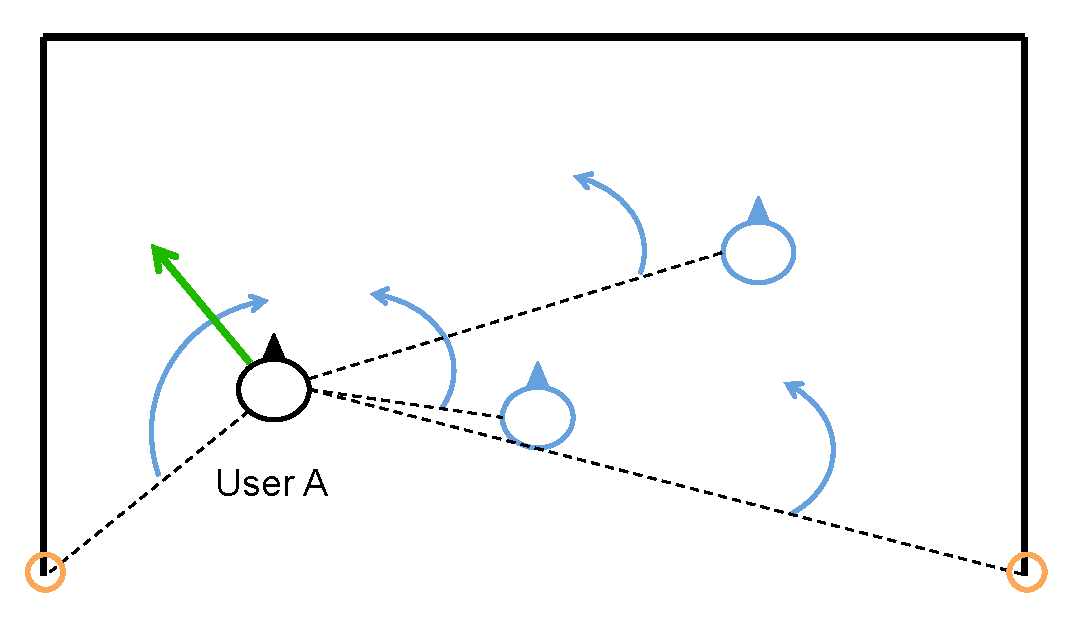
\includegraphics[width=.49\textwidth]{figures/ch5/pf_r_total}
  \caption{\label{fig:5_pf_total}The global translational and rotational potential field for user A in a three-wall CAVE.}
\end{figure}


To find the optimal configuration for a user in real time, we use an iterative method as presented in Algorithm~\ref{algo:optimal_point}. The idea is to create a virtual configuration $c(p,q)$ starting from user's current configuration $c_{u}(p_{u},q_{u})$ and is pushed by the sum of all potential fields step by step till we reach a certain precision $\epsilon_{T}$ ($\epsilon_{R}$) or a given maximum round number $n_{T}$ ($n_{R}$) - in case the algorithm does not converge in time. This allows us to find the optimal configuration for each user during a rendering frame.

\begin{algorithm}[htb]
\caption{Iterative function for optimal configuration computing.}
\label{algo:optimal_point}
\begin{algorithmic}
\REQUIRE $\epsilon_{T} \geq 0 \: \AND \: n_{T}>0 \: \AND \: \epsilon_{R} \geq 0 \: \AND \: n_{R}>0$
\STATE $p \leftarrow p_{u}$
\STATE $p_{opt} \leftarrow p+\sum \overrightarrow{ft}_{i}$
\STATE $round \leftarrow 0$
\WHILE{$|p_{opt}-p|>\epsilon_{T} \: \AND \: round<n_{T} \:$}
\STATE{$p \leftarrow p_{opt}$}
\STATE{$p_{opt} \leftarrow p+\sum \overrightarrow{ft}_{i}$}
\STATE{$round \leftarrow round+1$}
\ENDWHILE

\STATE $q \leftarrow q_{u}$
\STATE $q_{opt} \leftarrow q \cdot \sum fr_{i}$
\STATE $round \leftarrow 0$
\WHILE{$(q^{-1}_{opt} \cdot q).angle>\epsilon_{R} \: \AND \: round<n_{R} \:$}
\STATE{$q \leftarrow q_{opt}$}
\STATE{$q_{opt} \leftarrow q \cdot \sum fr_{i}$}
\STATE{$round \leftarrow round+1$}
\ENDWHILE
\RETURN $p_{opt}, q_{opt}$
\end{algorithmic}
\end{algorithm}


The potential fields constantly update optimal configurations for each user, we can use the difference between user's current configuration and corresponding optimal configuration to modify user's navigation control. Here we got two options:

\paragraph{Option 1: Scaling}
We can use the difference to scale user's input. For translation, the difference can be represented by a vector $\overrightarrow{d}$ pointing from the optimal position to user's current position. By splitting user's velocity $\overrightarrow{v_{u}}$ (and acceleration $\overrightarrow{a_{u}}$) to different axis, these components can then be scaled by the corresponding components of $\overrightarrow{d}$:   

\begin{equation}
\overrightarrow{v'_{ui}}=\overrightarrow{v_{ui}} \cdot (1+\frac{\overrightarrow{v_{ui}} \cdot \overrightarrow{d_{i}}}{|\overrightarrow{v_{ui}} \cdot \overrightarrow{d_{i}}|} \cdot K_{ot} \cdot |\overrightarrow{d_{i}}|), \;i\in\{x ,y\}
\end{equation}

where $K_{ot}$ is a coefficient to increase or reduce the influence of potential field. When $\overrightarrow{v_{ui}}$ is in the same direction with $\overrightarrow{d_{i}}$, the final input $\overrightarrow{v'_{ui}}$ will be amplified compared to $\overrightarrow{v_{ui}}$, otherwise it will be reduced (Figure~\ref{fig:5_option1:t}).

Similarly, for rotational control, we use $\theta$ to represent the angle between user's optimal orientation $q_{opt}$ and current orientation $q_{u}$. The angular velocity will be amplified if the user turns away from $q_{opt}$, otherwise it is reduced to encourage user's turn faster towards $q_{opt}$ (Figure~\ref{fig:5_option1:r}).

\begin{equation}
\omega'_{u}=\omega_{u} \cdot (1+sign \cdot K_{or} \cdot \theta),\;sign \in \{-1, 1\} 
\end{equation}

where $sign$ is computed depending on the relationship between user's angular velocity and the rotation direction starting from $q_{opt}$ to $q_{u}$. $K_{or}$ also serves as a scale factor like $K_{ot}$. Both $K_{ot}$ and $K_{or}$ are set small enough so the potential field will not inverse the direction of user's input.

\begin{figure}[htb]
  \begin{subfigure}{.5\textwidth}
    \centering
    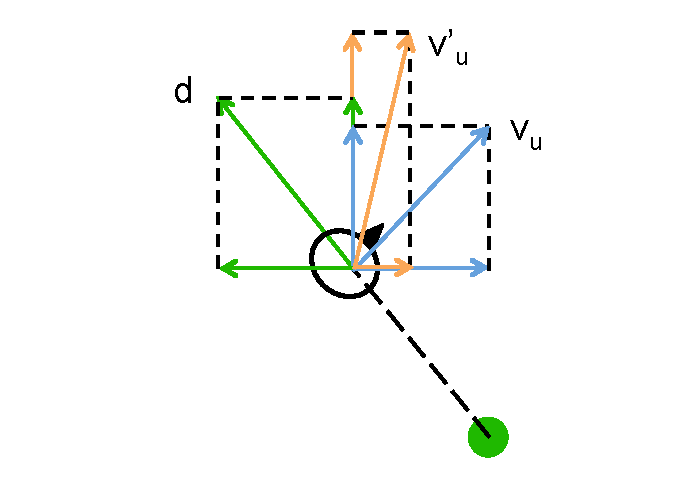
\includegraphics[height=5cm]{figures/ch5/option1_t}
    \caption{Velocity vectors are scaled by $\overrightarrow{d}$.}
    \label{fig:5_option1:t}
  \end{subfigure}
  \begin{subfigure}{.5\textwidth}
    \centering
    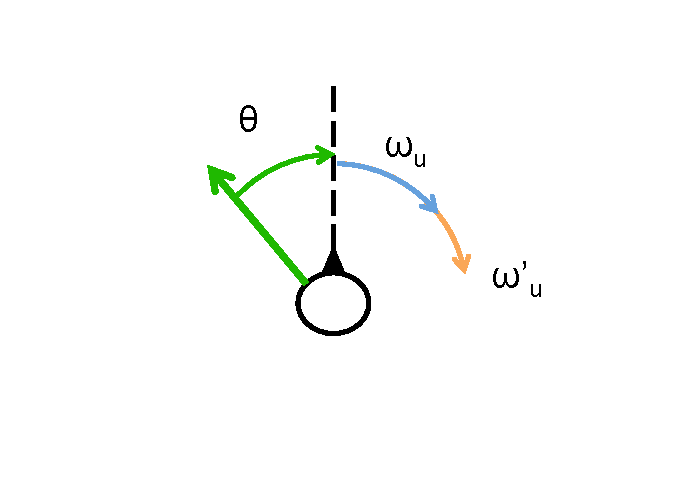
\includegraphics[height=5cm]{figures/ch5/option1_r}
    \caption{Angular velocity is scaled by $\theta$.}
    \label{fig:5_option1:r}
  \end{subfigure}
  \caption{\label{fig:5_option1}Scaling of user's input by the difference between user's current configuration and the optimal configuration.}
\end{figure}

\paragraph{Option 2: Acceleration Insertion}
Instead of scaling user's input, we can also insert additional accelerations to ``pull" users towards the optimal configuration. We can consider that the user and optimal configuration are connected by a mass spring damper system (a PD system in automatics which is useful to represent interconnection between two mobile entities). For translation, the total acceleration is the sum of acceleration coming from the transfer function $\overrightarrow{a_{u}}$ and $\overrightarrow{a_{o}}$ generated by the optimal position (Figure~\ref{fig:5_option2:t}). $\overrightarrow{a_{o}}$ is expressed as follows:

\begin{equation}
\overrightarrow{a_{o}}=K_{ot} \cdot (p_{u}-p_{o})+ B_{ot} \cdot (\overrightarrow{v_{u}}-\overrightarrow{v_{o}})
\end{equation}

where $K_{ot}$ and $B_{ot}$ are respectively spring and damper coefficients, $p_{o}$ and $\overrightarrow{v_{o}}$ are the position and velocity of the optimal configuration.

For rotation, the total angular acceleration $\dot{\omega}_{total}$ is the sum of $\dot{\omega}_{u}$ and $\dot{\omega}_{o}$ (Figure~\ref{fig:5_option2:r}). $\dot{\omega}_{o}$ is expressed as follows:

\begin{equation}
\dot{\omega}_{o}=K_{or} \cdot (q_{u}-q_{o})+ B_{or} \cdot (\omega_{u}-\omega_{o})
\end{equation}

where $K_{or}$ and $B_{or}$ are respectively spring and damper coefficients, $q_{o}$ and $\omega_{o}$ are the optimal orientation and its rotational velocity.

\begin{figure}[htb]
  \begin{subfigure}{.5\textwidth}
    \centering
    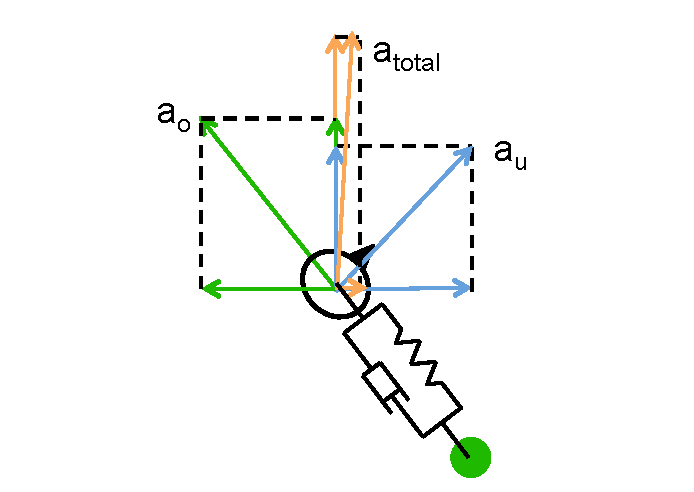
\includegraphics[height=5cm]{figures/ch5/option2_t}
    \caption{Additional linear acceleration $\overrightarrow{a_{o}}$.}
    \label{fig:5_option2:t}
  \end{subfigure}
  \begin{subfigure}{.5\textwidth}
    \centering
    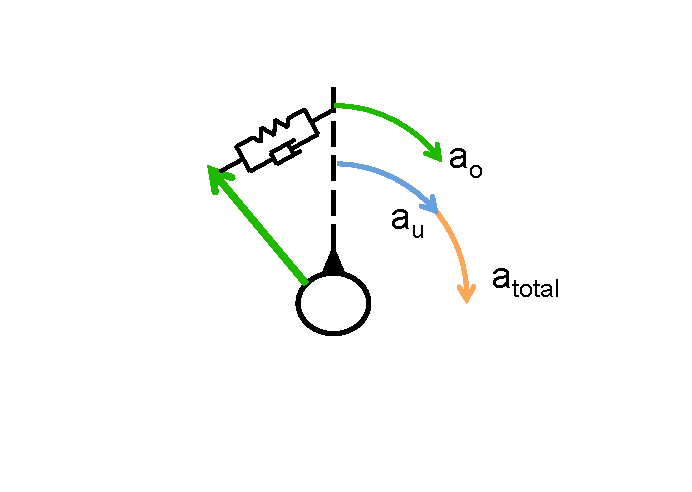
\includegraphics[height=5cm]{figures/ch5/option2_r}
    \caption{Additional angular acceleration $\dot{\omega}_{o}$.}
    \label{fig:5_option2:r}
  \end{subfigure}
  \caption{\label{fig:5_option2}Inserting additional accelerations by the difference between user's current configuration and the optimal configuration.}
\end{figure}

\paragraph{Comparison}
These two options give users similar navigation experiences in terms of perceived acceleration as they are both based on the difference between user's current configuration and the optimal configuration decided by the potential field distribution. The major difference is that option 2 continues to accelerate the navigation as long as the user is not at the optimal configuration, while with option 1, the vehicle is accelerated only when the user intends to move physically.

The principal of option 1 is that a static user should not be ``penalized" by the variation of surrounding potential fields caused by the movements of other users. This method assures the stability of users' control of the navigation speed, however, it does not guarantee that users stay always near their optimal configurations. On the contrary, option 2 introduces accelerations to restrain users to their optimal configurations so they will hardly enter critical situations. Consequently, users are never in a stable state outside their optimal configurations.

For now we keep both options in the dynamic model because they both have advantages and drawbacks. User studies are needed to identify appropriate parameters for each option and to compare their usability in terms of navigation efficiency and comfort.

\subsubsection{Command Configuration}
Since users are mobile in the physical workspace, the potential field for each user is changing all the time depending on the positions of other users, the movements of one user change instantaneously the optimal configuration of another, which will induce instability to the navigation control, especially for option 2.

To reduce this instability, a possible solution is to define a command configuration $c_{command}$ as an intermediate layer between $c_{u}$ and $c_{opt}$. The $c_{command}$ indicates where the user should be in the real world and tries to join $c_{opt}$ with a certain delay. For example, we can create a mass spring damper link between $c_{command}$ and $c_{opt}$ to reduce the influence of $c_{opt}$ on the virtual vehicle.

Moreover, the optimal configuration defined by the potential field may not always be the preferred destination as we may have some other real world constrains to take into account. For example, a user may need to leave more workspace for another user based on their individual task requirements. So the command configuration is useful as a higher abstraction level for us to integrate other real world constrains besides obstacles' potential fields. 


\subsection{Virtual World Constrains}
In most rate control navigation methods, the virtual vehicle is just a mobile reference frame whose position and orientation is directly set by user commands, so it can not be influenced by physical constrains defined in the virtual world (e.g. the vehicle can cross virtual objects like walls or floors). However, the dynamic vehicle defined in DYNAMIC receives user commands in form of accelerations, so forces in the virtual world could be easily applied to the vehicle by giving the vehicle a certain virtual mass.

\subsubsection{Interaction with Virtual World}
Various physical behaviors can be simulated when using the dynamic model to navigate in the virtual world:

\begin{itemize}
\item Viscosity of the virtual space or friction of the floor (add an acceleration in the opposite direction of the vehicle's current velocity).
\item Attraction or repulsion fields associated with a zone or a location (e.g. to stay within the boundary of the virtual scene or to show places of interest).
\item Collision with certain objects (e.g. a bounding box of virtual obstacles).
\end{itemize}

These physical interactions can be managed directly by the dynamic model that includes a simple physics engine, so the virtual world does not need to be physicalized. Otherwise, we can also associate the virtual vehicle to an entity in a physicalized virtual world to leave physical constrains to a separate physics engine.

\subsubsection{Interaction between Vehicles}
When multiple users navigate in the same virtual space with the dynamic model, physical links could be established between vehicles to allow different levels of navigation control:     

\begin{itemize}
\item Closely-coupled navigation: there is a rigid physical link between vehicles, one user's move will have an instant influence on the navigation of another. This is typical for object co-manipulation - when several users move together a heavy or large object to another place.
\item Loosely-coupled navigation: there is a soft physical link between vehicles. For example, a user's vehicle is attached to the vehicle of another user by a spring so the former could be guided from one place to another while keeping a certain degree of autonomy.
\item Individual navigation: no physical constrains exist between different vehicles.
\end{itemize}

Users can switch from one navigation state to another by changing the physical link connecting the vehicles (Figure~\ref{fig:5_user_inter}). Consequently, the dynamic navigation model broadens supported collaborative scenarios in multi-user immersive virtual environment by enabling these different navigation states. Moreover, the interaction between vehicles provides an automatic way for co-located users to switch from one collaborative mode to another. For example, when users navigate to the same place from different virtual locations, soft links can be added once they arrive to help them enter consistent collaborative mode by guiding their vehicles to specific configurations.

\begin{figure}[htb]
  \centering
  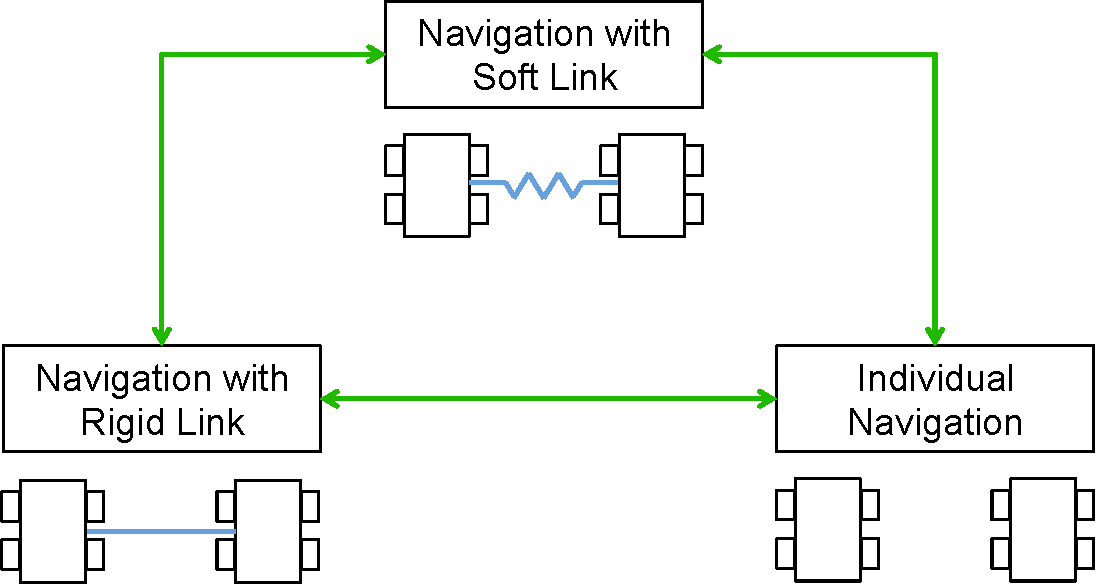
\includegraphics[width=.8\textwidth]{figures/ch5/user_inter}
  \caption{\label{fig:5_user_inter}Three levels of interactive navigation control (example of two vehicles).}
\end{figure}


% -------------------------------------------------------------------------------------------------

\section{Implementation}
In this section, we explained how we put concepts described above together into a functional model, and how we created specific data structure to store all kinematic information of users and their vehicles. Finally, we presented an object-oriented design of the model with detailed descriptions of main components.

\subsection{Control Process}
In virtual reality applications, the general program loop contains three steps: user input collection, logic processing and rendering update. As shown in Figure~\ref{fig:5_process}, depending on user's input, the dynamic model computes withs its three main components the accelerations to apply to the virtual vehicle.

\begin{figure}[htb]
  \centering
  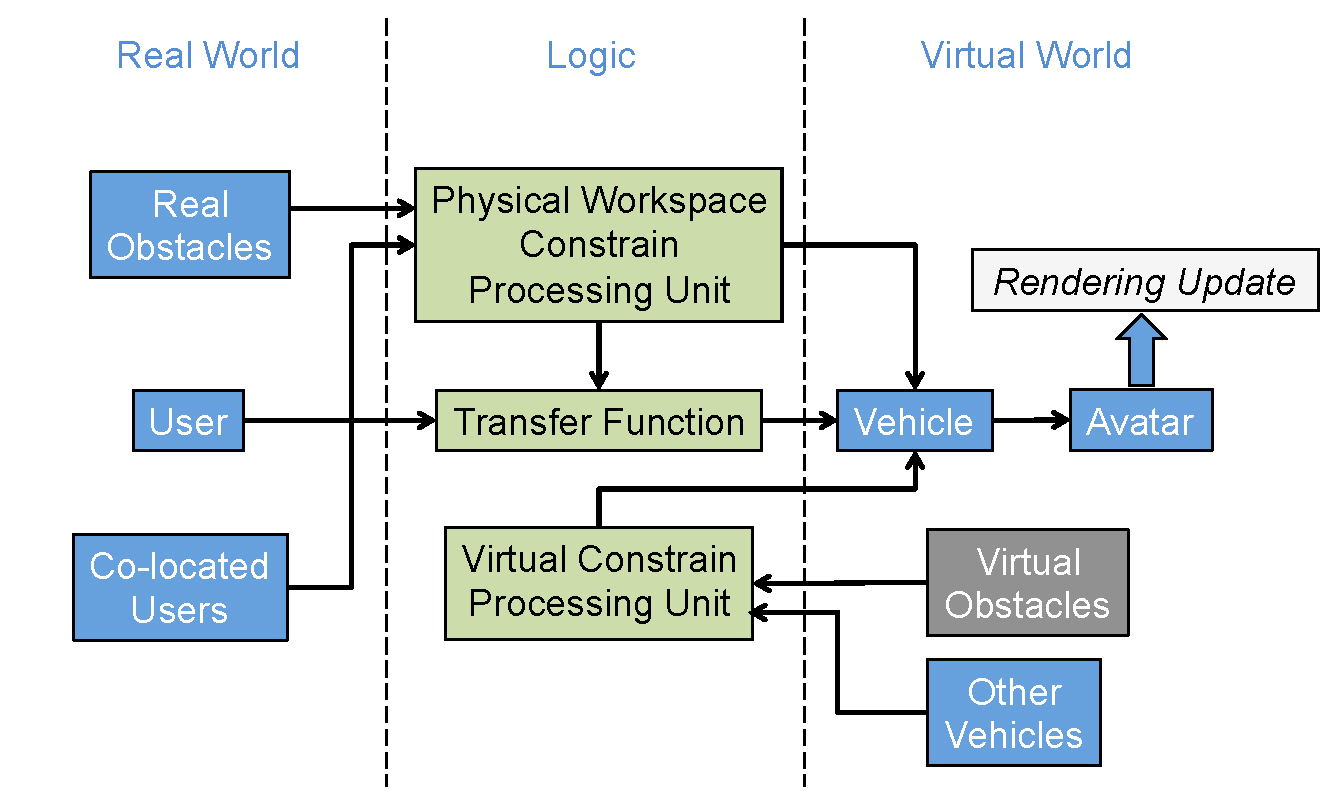
\includegraphics[width=.9\textwidth]{figures/ch5/process}
  \caption{\label{fig:5_process}The general control process of DYNAMIC.}
\end{figure}

Since we defined two options to integrate the influence of potential fields (section~\ref{sec:5_solution}), there are two corresponding ways to compute the total acceleration for the vehicle. If we name $acc_{user}$ the acceleration (both linear and angular components) generated from the transfer function, $acc_{obs}$ from the potential field, and $acc_{vir}$ the one from virtual constrains, the total acceleration $acc_{total}$ for option 2 can be expressed as:

\begin{equation}
acc_{total}=acc_{user}+acc_{obs}+acc_{vir}
\end{equation}

While for option 1, the potential field scales $acc_{user}$ instead of inserting an additional acceleration, so we get:

\begin{equation}
acc_{total}=scale(acc_{user},\: (\overrightarrow{d},\theta))+acc_{vir}
\end{equation}

where $\overrightarrow{d}$ and $\theta$ represent the difference between user's current configuration and the optimal configuration decided by the potential field distribution.

With the total acceleration $acc_{total}$ and the vehicle's configuration $c_{veh}$ in the previous frame, we can get a new $c_{veh}$ to correctly position user's corresponding stage and avatar in the virtual world to get proper rendering results.


\subsection{Data Structure}
In this dynamic model, we often need different kinds of kinematic information about an object such as its velocity and acceleration, along with its static configuration to control the virtual navigation. In 3D space, an object's kinematic state contains two parts of information respectively for translation and rotation, except for points (considered as particles) that have only positional information. 

So we created a variable named KS (kinematic state) to assemble all motion-related data of a given object and implement corresponding rules to update it in each frame. Table~\ref{tab:5_ks_components} lists different components of an object's KS.

\begin{table}[hbt]
\renewcommand{\arraystretch}{1.3}
\caption{Components of an object's KS}
\label{tab:5_ks_components}
\centering
\begin{tabular}{l l l}
  \hline
  Components & Translation Part & Rotation Part \\
  \hline
  Configuration $c(p, q)$ & $p(x, y, z)$ & $q(w, x, y, z)$ \\
  Velocity $v(\overrightarrow{v}, \omega)$ & $\overrightarrow{v}(v_{x}, v_{y}, v_{z})$ & $\omega(\omega_{x},\omega_{y},\omega_{z})$ \\
  Acceleration $a(\overrightarrow{a}, \dot{\omega})$ & $\overrightarrow{a}(a_{x}, a_{y}, a_{z})$ & $\dot{\omega}(\dot{\omega}_{x},\dot{\omega}_{y},\dot{\omega}_{z})$ \\
  \hline
\end{tabular}
\end{table}

The translation part $(p,\overrightarrow{v},\overrightarrow{a})$ is expressed in vectors, while we represent the rotation part by quaternion and Euler angles $(q,\omega,\dot{\omega})$. Quaternion is a convenient math tool to express spatial rotations (or orientation relative to a reference frame), but is a little complicated to get its derivatives, so instead, angular velocity and acceleration are stored using Euler angles.

An object's KS changes constantly while moving in 3D space. Typically, in the virtual world, we can animate an object by injecting a new acceleration on it to modify its current KS, which will result in a corresponding velocity and configuration change. However, the KS of a real world entity located by optical tracking (e.g. a user's body) will be directly updated by getting a new static configuration. Implementation details about KS update can be found in Appendix~\ref{appendix:ks}. 


\subsection{Components}
We implemented a first version of DYNAMIC with Python for BlenderVR (Appendix~\ref{appendix:platform}), and it can be easily ported to other object-oriented languages. Figure~\ref{fig:5_uml} is a UML class diagram of DYNAMIC (omitting interfaces that communicate with codes managing user input and rendering).

\begin{figure}[htb]
  \centering
  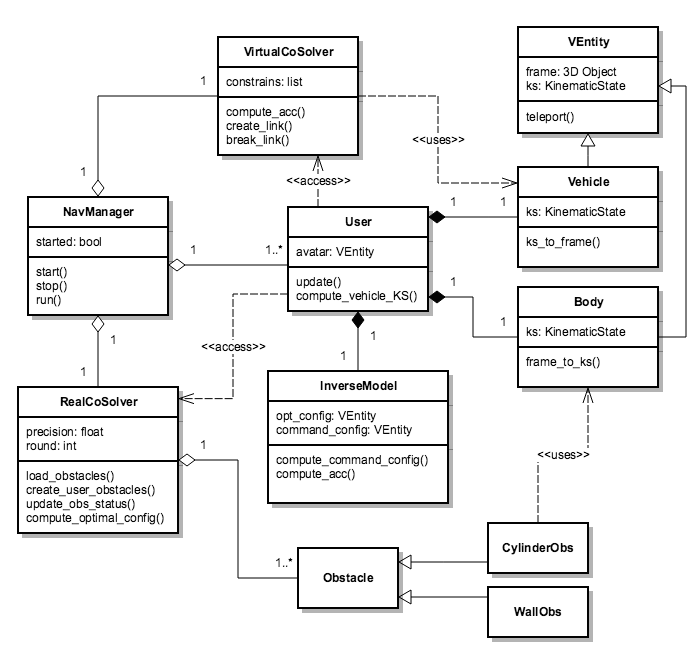
\includegraphics[width=.9\textwidth]{figures/ch5/uml}
  \caption{\label{fig:5_uml}The UML class diagram of DYNAMIC.}
\end{figure}


Here we give explanations to a list of main components (in form of classes) that constitute the model:

\begin{itemize}
\item \textit{NavManager}: The main class of the navigation model that contains a list of users and constrain solvers, it initiates calls to transfer function of each user and to functions defined in these solvers. The navigation can be activated or deactivated through a control boolean.
\item \textit{VEntity}: A basic class used to represent a virtual entity involved in the simulation. Each virtual entity has its own KS, and eventually a mesh for visualization in the virtual world. For example, the \textit{Vehicle} and \textit{Body} (user's physical body in the real world) are all inherited classes of \textit{VEntity}. A virtual entity's initial configuration can be set by ``teleportation" without affecting other KS properties.
\item \textit{User}: A class groups all user-related information and combines accelerations from different sources to compute a new KS for the corresponding vehicle.
\item \textit{RealCoSolver}: A \textit{Real Constrain Solver} that manages constrains from the physical workspace by computing an optimal configuration for each user.
\item \textit{InverseModel}: A unit contained in each user that manages the command configuration and implements option 1 or option 2 mentioned in section~\ref{sec:5_solution}.
\item \textit{VirtualCoSolver}: A \textit{Virtual Constrain Solver} that processes a list of constrains defined in the virtual world. It creates or breaks the physical link between a pair of vehicles and computes accelerations accordingly. 
\end{itemize}

% -------------------------------------------------------------------------------------------------

\section{Discussion}

The dynamic model constitutes a framework for co-located immersive collaboration and it possesses the following characteristics:

The model is \textbf{generic}. First, it can be applied to most popular immersive systems regardless of the behavioral interface instantiation: whether the visual immersion is provided by CAVE-like system or HMDs, whether the available physical workspace is large or small, etc. Second, it can also help users to avoid mobile obstacles in real time, all tracked users and objects present in the physical workspace can be integrated into the cohabitation management process. At last, the management of constrains from the physical workspace and virtual world is independent with the navigation transfer function, it can be easily adapted to work with other navigation techniques like walking or steering metaphors.

The model is \textbf{extensible}. Unlike the Altered Human Joystick, this dynamic model can support from one to several users without setting specific zones for each user, users can enter or leave the immersive system during the simulation. Additionally, constrains with more degrees of freedom (DoF) can be included for 6DoF virtual navigation, for example, user's field of view should be constrained between the top and bottom borders of screens to assure visual immersion. Moreover, this model could be extended to manage the coexistence of users and robotic devices during immersive collaboration. For example, the Scale 1\texttrademark{} (Figure~\ref{fig:1_hi:scale1}) is a robotic arm that can move with the user in control to provide haptic feedback over a large workspace. Our dynamic model can not only help other co-located users to avoid colliding with the arm (the arm is considered a mobile obstacle), but also be extended to make the arm to ``be aware of" the positions of users when moving inside the shared physical workspace.

With the concepts and code structure described above, we implemented a first version of DYNAMIC with parameters that are configured empirically according to the configuration (form and size) of our immersive system. Further studies are required to achieve a more efficient and robust navigation model.

In term of users' comfort, an important question is that in general, how we can find appropriate parameters (e.g. gain value for the transfer function and the inverse model) for this dynamic model, considering that each user has his/her own way to use the navigation metaphor and does not have the same reaction to system-induced accelerations. So whether do we need a calibration process to identify parameters for each user, or can we find parameters that correspond to a generic model describing human reaction to accelerations? Another question is how we can limit the perceived accelerations due to obstacles in physical workspace. Can we find a threshold under which a user will not feel the additional accelerations? Or at least does not find it disturbing for the navigation control?

To answer these questions, follow-up user studies are needed to test different parameters under various conditions and to improve the model according to users' feedbacks.

% -------------------------------------------------------------------------------------------------

\section{Conclusion}
In this last chapter, we presented a novel dynamic navigation model named DYNAMIC - a generalized version of the Altered Human Joystick metaphor that we designed for co-located collaboration in multi-user immersive systems. On the one hand, this model integrates constrains from physical workspace by a potential field method to solve user cohabitation problems. On the other hand, it takes into account constrains coming from the virtual world to enable interactive control of a user's vehicle and interactions between users.

This model offers a generic solution for user cohabitation in terms of user number and geo\-metric properties of the immersive system, and enables different interactive navigation levels between users. Based on the current implementation, further studies can be conducted to refine this model regarding user comfort during navigation control and to include more types of devices for immersive collaboration.